\documentclass[a4paper, 12pt,]{scrartcl}



\usepackage[utf8]{inputenc}

\usepackage[ngerman]{babel}
\usepackage{amssymb}
\usepackage[T1]{fontenc}
\usepackage{mathtools}
\usepackage{amsmath}
\usepackage{ntheorem}
\usepackage{bbm}
\usepackage{dsfont}
\usepackage{color}
\usepackage{slashed}
\usepackage{esint}
\usepackage{graphicx} 
\usepackage{bm}
\usepackage{mathabx}
\usepackage{changepage}
\usepackage{subcaption}
\usepackage{float}
\usepackage{mwe}
\usepackage{multirow}
\usepackage{hyperref}
\usepackage{cleveref}
\begin{document}


\begin{titlepage}
	\centering
	{\scshape\LARGE Universität Tübingen \par}
	\vspace{2cm}
	{\huge\bfseries Transformator \par}
	\vspace{2cm}
	{\Large \scshape Blockpraktikum 2021} \par
	\vspace{2cm}
	{\Large  Erste Version} \par
	\vspace{2cm}
	{\Large\itshape \underline{Christian Gommeringer} \space \space  \underline{Matthias Gatter}\par}
	\vfill 
	{\large betreut von Dr. Hehl}
	\vfill

	{\large \today\par}
\end{titlepage}
\newpage 
\tableofcontents 

\newpage
\section{Einleitung}
\begin{flushleft}


\end{flushleft}
% > < | 

\section{Theorie}
Um die Theorie für die Funktionsweise eines Transformators zu verstehen, wiederholen wir zunächst die Gesetzmäßigkeiten der Induktion. Die Maxwell Gleichungen enthalten für einen konstanten elektrischen Strom (E=konst.) die Beziehung
\begin{equation*}\text{rot}\,\vec{B}=\mu_0\,\vec{j}\end{equation*}
was sich über Integration und Anwendung des Satzes von Stokes zu
\begin{equation}\oint\vec{B}\,\text{d}\vec{s}=\mu_0\label{e1}\end{equation}
Über diese Gleichung kann über die Annahme, dass das Magnetfeld innerhalb einer Spule konstant in deren Längsrichtung zeigt und außerhalb Null ist, das Magnetfeld einer Spule berechnet werden.
\begin{align*}l\,B=N\,\mu_0\,I\\
\Rightarrow\;B=\mu_0\,\frac{N}{l}\,I\end{align*}
Hierbei ist $l$ die Länge der Spule und N die Anzahl ihrer Windungen. Wenn sich die Spule in einem Medium befindet, modifiziert sich die Gleich leicht zu $B=\mu_0\mu_r\,N/l\,I$. Durch einfügen eines Mediums mit $\mu_r>1$ in das Spuleninnere, kann also das Magnetfeld vergrößert werden.
Nach der Induktionsgleichung
$$\text{rot}\,\vec{E}=-\frac{\partial{B}}{\partial{t}}$$
was wieder zu
\begin{equation}\oint\vec{E}\,\text{d}\vec{s}=\frac{U}{N}=-\frac{\partial}{\partial{t}}\int\vec{B}\,\text{d}\vec{f}\label{e2}\end{equation}
In unserem Fall der Spule lässt sich dies auswerten zu
\begin{align}U&=-N\,\dot{B}\,A=-\mu_0\mu_r\,\frac{N^2\,A}{l}\,\dot{I}\notag\\
&=:\,{-L}\,\dot{I}\label{e3}\end{align}
Das ist das bekannte Induktionsgesetz mit der Induktivität L. A ist hier die Querschnittsfläche der Spule. In dem betrachteten Fall handelt es sich um die Selbstinduktion. Für die induzierte Spannung die eine Spule 1 in einer Spule 2 induziert ergibt sich die Beziehung.
$$L_{12}=\mu_0\mu_r\,\frac{N_1\,N_2\,A}{l_1},$$
wobei vorausgesetzt wurde, dass die 2. Spule senkrecht und vollständig vom Magnetfeld der 1. Spule durchsetzt wird. Ist dies nicht der Fall muss noch ein oft experimentell zu bestimmender Kopplungsfaktor $k\in[0,1]$ einführt, der dann die wahre Gegeninduktivität $L_{12,r}$ erzeugt.
$$L_{12,r}=k\,L_{12}$$
Für den idealen Transformator ist $k=1$, und auch ansonsten werden keine zusätzlichen Effekte, oder Widerstände berücksichtigt. Im Fall, dass der Stromkreis der zweiten Spule nicht geschlossen ist und somit kein Strom fließt, sondern nur die Spannung abgegriffen wird, wird das Magnetfeld der Spule nur durch den Strom $I_1$ durch Spule 1 erzeugt, und somit gilt für die induzierte Spannung, die an den beiden Spulen anliegt
\begin{align*}U_1\coloneq{U_{\text{ind},1}}=-L_{11}\,I_1\\
U_2\coloneq{U_{\text{ind},2}}=-L_{12}\,I_1\\
\Rightarrow\,\frac{U_1}{U_2}=\frac{L_{11}}{L_{12}}=\frac{N_1}{N_2}=:\gamma\end{align*}
mit der so definierten Übertragungszahl $\gamma$.\newline
In einem realen Transformator sind noch zusätzliche Effekte zu berücksichtigen. Die elektrischen Leitungen besitzen natürlich Widerstände, was unter dem Begriff Kupferverluste zusammengefasst wird. Außerdem wird in die Spulen eines realen Transformators ein ferromagnetisches Material eingefügt, um den magnetischen Fluss zu erhöhen. Durch die Ummagnetisierung dieses Materials, bedingt durch den Wechselstrom, wird Wärme frei. Des Weiteren werden durch  die sich ändernden Magnetfelder Wirbelströme induziert, die über den elektrischen Widerstand auch Leistung abführen. Dieser Effekt dadurch verringert, das man das Material in möglichst kleine Segmente unterteilt, die nichtleitend mit einander verbunden sind. Die Energieverluste durch Hysterese und die induzierten Wirbelströme werden unter dem Begriff Eisenverluste zusammengefasst.\newline\newline
%\begin{figure}[H]\centering\includegraphics[scale=0.8]{}\caption{ausführliches Ersatzschaltbild des realen Transformators}\end{figure}
Diese Effekte können auch durch typische elektrische ideale Bauelemente in einem Ersatzschaltbild modelliert werden. Man findet darin einen idealen Übertrager mit Übersetzungsverhälnis $\gamma$. Dessen Model erläutere ich zunächst kurz. Im folgenden nehmen wir an, dass $L_{12}=L_{21}=:M$. Fließen durch beide Spulen Ströme $I_1$ und $I_2$, wobei im sekundären Stromkreis ein Widerstand Z zugeschaltet sei, so ergeben sich die Spannungen zu
\begin{align}\label{e4}U_1&=i\,\omega\,L_1\,I_1-i\,\omega\,M\,I_2\\
U_2&=i\,\omega\,M\,I_1-i\,\omega\,L_2\,I_2\label{e5}\end{align}
Hierbei sind die Vorzeichen so gewählt, dass beim Unbelasteten Transformator beide Spannungen das selbe Vorzeichen haben. Zur Ableitung des idealen Übertragers bleiben wir im Modell streuungsfreien Transformators. Es gilt also $M=\sqrt{L_1\,L_2}$. Damit bleibt das Spannungsverhältnis ideal
\begin{align*}\frac{U_1}{U_2}&=\frac{L_1\,I_1-M\,I_2}{M\,I_1-L_2\,I_2}=\frac{\frac{L_1}{L_2}\,I_1-\frac{M}{\sqrt{L_1\,L_2}}\,\sqrt{\frac{L_1}{L_2}}\,I_2}{\frac{M}{\sqrt{L_1\,L_2}}\,\sqrt{\frac{L_1}{L_2}}I_1-I_2}\\
&=\frac{\frac{L_1}{L_2}\,I_1-\sqrt{\frac{L_1}{L_2}}\,I_2}{\sqrt{\frac{L_1}{L_2}}I_1-I_2}=\sqrt{\frac{L_1}{L_2}}\end{align*}
Für die Ströme gilt
$$I_2=\frac{i\,\omega\,M}{Z+i\,\omega\,L_2}\,I_1=\sqrt{\frac{L_1}{L_2}}\,\frac{M}{\sqrt{L_1\,L_2}}\,\frac{i\,\omega\,L_2}{Z+i\,\omega\,L_2}$$
Im Fall des idealen Übertragers lässt man nun die Induktivitäten gegen unendlich gehen $L_1,L_2\rightarrow\infty$, während $\sqrt{L_1/L_2}=\gamma=konst.$ und $M/\sqrt{L_1\,L_2}=1$ gelassen wird, um dadurch folgende Relationen zu erhalten
\begin{align}\label{e6}\frac{U_1}{U_2}&=\sqrt{\frac{L_1}{L_2}}=\frac{N_1}{N_2}=\gamma\\
\frac{I_1}{I_2}&=\sqrt{\frac{L_2}{L_1}}=\frac{1}{\gamma}\label{e7}\end{align}
Daraus ergibt sich zusätzlich
\begin{equation}\frac{U_1}{I_1}=\gamma^2\,\frac{U_2}{I_2}=\gamma^2\,Z\label{e8}\end{equation}
Somit wirkt der Widerstand auf der Sekundärseite wie ein das $\gamma^2$-fache eines Widerstands auf der Primärseite. Wenn wir nun die Gleichungen \cref{e4} und \cref{e5} umformen und noch ein interne Widerstände $R_{i1},R_{i,2}$ sowie einen Lastwiderstand $R_L$ einführen, erhalten wir
\begin{align}\label{e9}U_1&=R_{i,1}\,I_1+i\,\omega\,\left(L_1-\gamma\,M\right)\,I_1+i\,\omega\,\gamma\,M\,\left(I_1-\frac{I_2}{\gamma}\right)\\
-\gamma\,U_2&=-\gamma\,R_L\,I_2=\gamma^2\,R_{i,2}\,\frac{I_2}{\gamma}+i\omega\,\left(\gamma^2\,L_2-\gamma\,M\right)\,\frac{I_2}{\gamma}+i\,\omega\,\gamma\,M\left(\frac{I_2}{\gamma}-I_1\right)\label{e10}\end{align}
$U_2$ Ist hier also die Spannung am Lastwiderstand. Diese Gleichungen können auch in eine Schaltung überführt werden, wobei Spannung 2 zwischen den Punkten 2 und 2' anliegt und dann über den idealen Übertrager auf die Sekundärseite übertragen wird. In der Masche 2 fließt der Strom $I_2/\gamma$. Diese Schaltung gibt exakt das wieder, was auch aufgrund der physikalischen Theorie transferiert würde.
\begin{figure}[H]\centering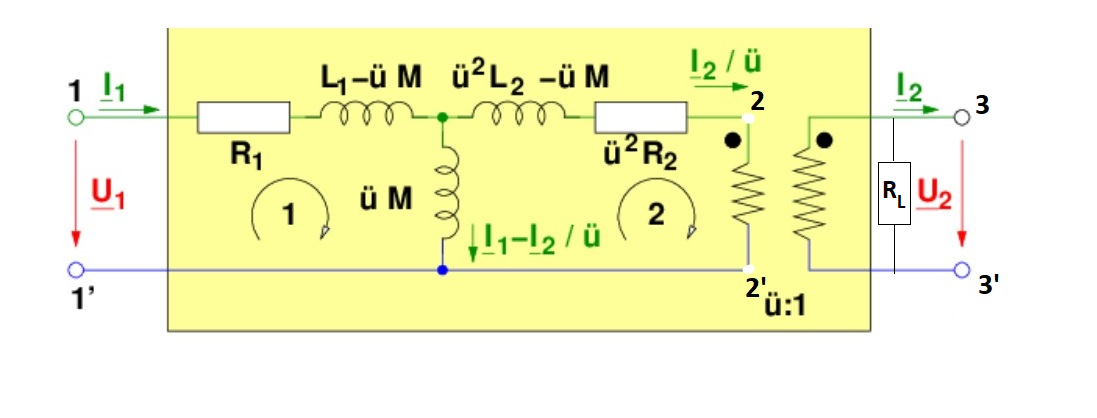
\includegraphics[scale=0.7]{ESB1'}\caption{Ersatzschaltbild für Gleichungen \ref{e4} und \ref{e5}; Quelle: http://www.ktet.fh-muenster.de/lehre/gde\_3.htlatex/gde\_3se37.html}\end{figure}
Wenn wir das streuungfreie Modell verlassen sind Gleichungen \ref{e4} und \ref{e5} sowie das Schaltbild uneingeschränkt richtig es gilt nun nur
\begin{align*}\frac{M}{\sqrt{L_1\,L_2}}&=k\\
\Rightarrow\; \gamma\,M&=k\,L_1=:L_h\\
\frac{1}{\gamma}\,M=k\,L_2\end{align*}
und damit
\begin{align*}
L_1-\gamma\,M&=(1-k)\,L_1=:L_{\sigma,1}\\
\gamma^2\,L_2-\gamma\,M&=\gamma^2\,(1-k)\,L_2=:\gamma^2\,L_{\sigma,2}\end{align*}
Wenn man nun noch die erwähnten Eisenverluste durch einen parallel geschalteten Widerstand $R_{E}$ berücksichtigt lässt sich das Ersatzschaltbild auch folgendermaßen schreiben, wobei sich die gestrichenen Größen durch $R_2'=\gamma^2\,R_{i,2}$, $L_{\sigma,2}'=\gamma^2\,L_{\sigma,2}$, sowie $R_1=R_{i,1}$ ergeben.
\begin{figure}[H]\centering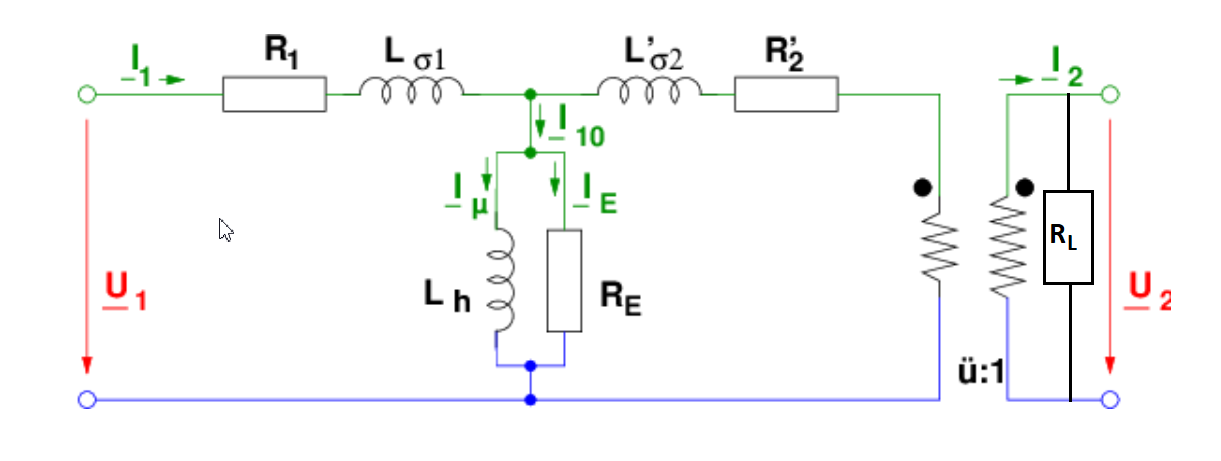
\includegraphics[scale=0.6]{ESB2'}\caption{vollständiges Ersatzschaltbild unter Berücksichtigung der Eisenverluste; \newline
Quelle: http://www.ktet.fh-muenster.de/lehre/gde\_3.htlatex/gde\_3se39.html}\end{figure}
Ebenso wie hier gezeigt, kann man die Ersatzschaltung auch auf die Sekundärseite verlagern, indem man die Gleichungen \ref{e4} und \ref{e5} folgendermaßen umschreibt.
\begin{align}\frac{U_1}{\gamma}&=\frac{1}{\gamma^2}\,R_{i,1}\,\gamma\,I_1+i\,\omega\,\left(\frac{1}{\gamma^2}\,L_1-\frac{1}{\gamma}\,M\right)\,\gamma\,I_1+i\,\omega\,\frac{1}{\gamma}\,M\,\left(\gamma\,I_1-I_2\right)\\
-U_2&=-R_L\,I_2=R_{i,2}\,I_2+i\,\omega\,\left(L_2-\frac{1}{\gamma}\,M\right)\,I_2+i\,\omega\,\frac{1}{\gamma}\,M\,\left(I_2-\gamma\,I_1\right)\end{align}
Aus diesen Gleichungen lässt sich ein äquivalentes Ersatzschaltbild zeichnen, wenn man $R_{i,1}'=\frac{1}{\gamma^2}\,R_{i,1}$, $L_{\sigma,1}'=\frac{1}{\gamma^2}\,L_{\sigma,1}$, $L_M=\frac{1}{\gamma^2}\,L_h$, sowie $R_{Fe}=\frac{1}{\gamma^2}\,R_{E}$ definiert ($U_1'=1/\gamma\,U_1$, $I_1'=\gamma\,I_1$).
\begin{figure}[H]\centering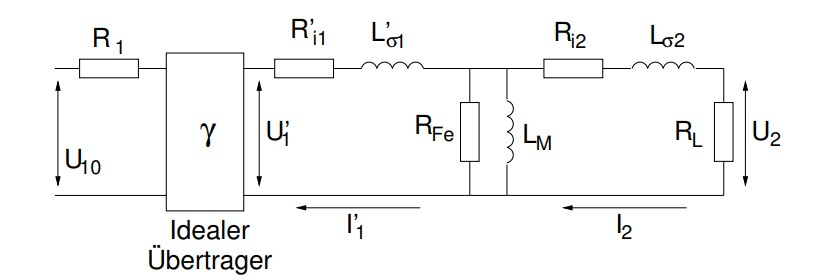
\includegraphics[scale=0.6]{ESB3}\caption{alternatives vollständiges Ersatzschaltbild unter Berücksichtigung der Eisenverluste; Quelle: Versuchsanleitung}\end{figure}
Wenn man nun $R_{i,1}'$ und $L_{\sigma,1}'$ gegenüber $R_{Fe}$ und $L_M$ vernachlässigt kann dies noch einmal vereinfacht werden
\begin{figure}[H]\centering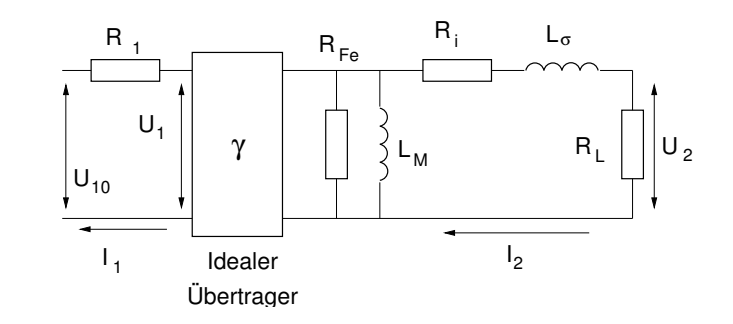
\includegraphics[scale=0.6]{ESB4}\caption{vereinfachtes Ersatzschaltbild; Quelle: Versuchsanleitung}\end{figure}
Der Widerstand $R_1$ in den letzten beiden Schaltbildern soll lediglich verdeutlichen, dass die Spannung, die am idealen Übertrager anliegt, über diesen Widerstand variiert werden kann.

\section{Versuchsdurchführung}
Im ersten Teil des Versuchs messen wir die Spannung die an der Sekundärseite des Trafos anliegt für verschiedene Eingangsspannungen, während keine Last an die sekundärseitigen Spule angeschlossen ist und kein Strom $I_2$ fließt. Dafür verstellen wir den Widerstand $R_1$ von 0 bis $100\,k\Omega$. Wir messen die Effektivwerte von $U_1$, $I_1$ und $U_2$ sowie die Phasenverschiebung $\varphi_1$ zwischen $U_1$ und $I_1$.\newline\newline

Im zweiten Teil des Versuchs halten wir die Eingangsspannung $U_1$, die so gemessen wird, wie es in Abbildungen 3 und 4 gezeichnet ist, konstant und variieren in einem großen Bereich vom Kurzschluss bis zum maximalen Wert den Lastwiderstand. Der konstante Eingangsstrom ist danach gerichtet, dass der sekundäre Kurzschlussstrom $2\,A$ nicht überschreitet. Wir messen Effektivwerte von $U_1$, $I_1$,$I_2$ und $U_2$ sowie die Phasenverschiebung $\varphi_1$ zwischen $U_1$ und $I_1$. Wir betreiben einen Transformator mit drei Spulen. Wir messen zusätzlich noch die Spannung, die an Spule 3 anliegt ohne Strom $I_3$, um ein Maß für den Fluss im Innern der Spule zu haben.

\section{Auswertung}
In unserer ersten Messung maßen wir die Spannung $U_2$ im Leerlauf. Dies entspricht dem Fall, in dem der Lastwiderstand einen unendlich großen Wert annimmt. Für die Spannung $U_2$ ergibt sich dadurch
$$U_2=\lim_{R_L\to\infty}\,\frac{R_L}{R_L+R_i+i\,\omega\,L_{\sigma}}\,U1'=U_1'=\frac{1}{\gamma}\,U_1,$$
wobei ich das vereinfachte Ersatzschaltbild verwendet habe. Über $R_{Fe}$ und $L_M$ fließt jedoch Strom und wird Leistung abgegeben. Es gilt
\begin{align*}\bar{P}_1=&\bar{U_1\,I_1}=\bar{U}_1\,\bar{I}_1\,\cos\varphi_1\\
=&\frac{1}{|Z_2|}\,\bar{U}_2^2\,\cos(\text{arg}(Z_2))\end{align*}
mit 
$$Z_2=\left(\frac{1}{R_{Fe}}+\frac{1}{i\,\omega\,L_M}\right)^{-1}$$
Es gilt 
\begin{align*}|Z_2|&=\frac{\bar{U}_2^2}{\bar{U}_1\,\bar{I}_1}\\
\text{arg}(Z_2)=\pm\varphi_1\end{align*}
Und damit lassen sich die fehlenden Größen berechnen.
\begin{align*}\frac{1}{R_{Fe}}&=\frac{1}{|Z_2|}\,\cos(\text{arg}(Z_2))=\frac{\bar{U}_1\,\bar{I}_1}{\bar{U}_2^2}\,\cos\varphi_1\\
L_M&=\frac{|Z_2|}{\omega\,\sin(\text{arg}(Z_2))}=\frac{\bar{U}_2^2}{\omega\,\bar{U}_1\,\bar{I}_1\,\sin\varphi_1}\end{align*}
In unserer Messung wurde der sogenannte Leistungsfaktor $\cos\varphi_1$ auf eine negative Zahl gemessen. Wie die obige Gleichung zeigt, kann dies nicht sein, da sonst der Widerstand negativ sein müsste, was nicht mit dem Ohmschen Gesetz vereinbar wäre. Es ist deshalb anzunehmen, dass Stromstärke und Spannung in verschiedene Richtungen gemessen wurde und dadurch das negative Vorzeichen zustande kam. Der Winkel muss entsprechend $\varphi_1\rightarrow\,\pi-\varphi_1$ umgerechnet werden. Dies ist besonders bei der zweiten Messung zu beachten.\newline
Die Messung der Effektivwerte von $U_1$, $I_1$, $U_2$ und $\varphi_1$ sind in folgenden Diagrammen dargestellt.
\begin{figure}[H]\centering
\begin{adjustwidth}{-1em}{7em}
  \begin{subfigure}[b]{0.5\textwidth}
    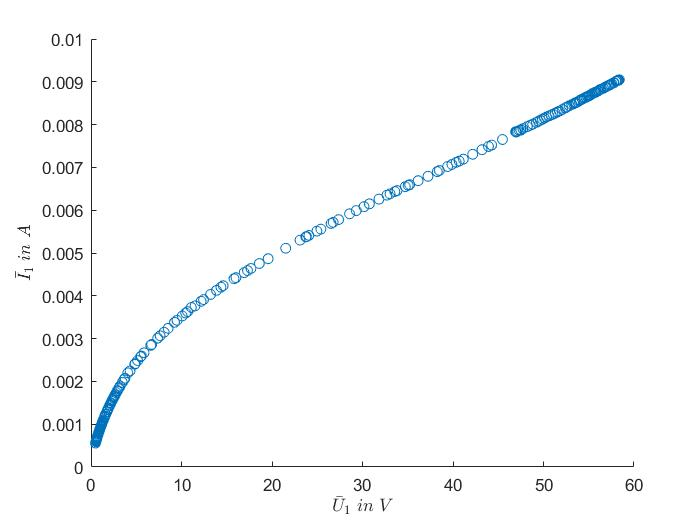
\includegraphics[width=\textwidth]{U1I11}
    \caption{Der Effektivwert der Stromstärke $\bar{I}_1$ in Abhängigkeit des Effektivwerts der Spannung $\bar{U}_1$}
    \label{fig:}
  \end{subfigure}
  %
  \begin{subfigure}[b]{0.5\textwidth}
    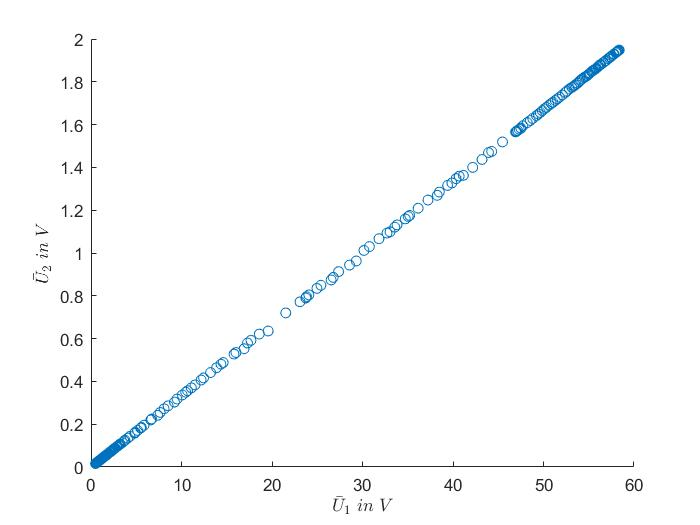
\includegraphics[width=\textwidth]{U1U21}
    \caption{Effektivwert der Spannung $\bar{U}_2$ in Abhängigkeit des  Effektivwerts der Spannung $\bar{U}_1$}
    \label{fig:}
  \end{subfigure}
\end{adjustwidth}\centering
\begin{adjustwidth}{-1em}{7em}
  \begin{subfigure}[b]{0.5\textwidth}
    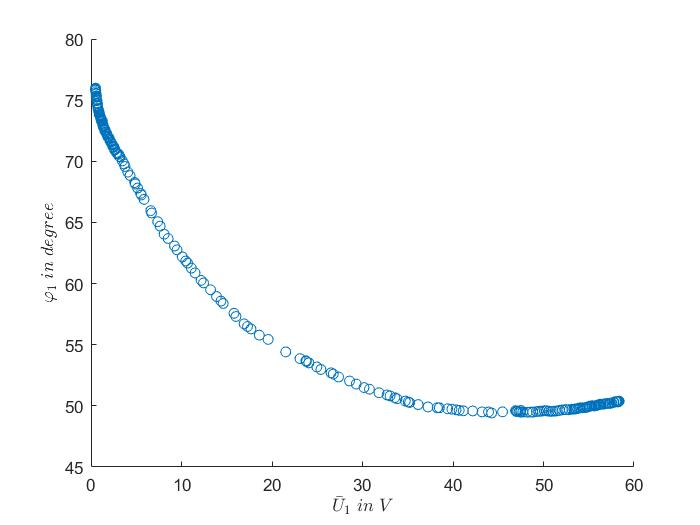
\includegraphics[width=\textwidth]{U11phi11}
    \caption{Phasenverschiebung zwischen Eingangsstrom und Eingangsspannung in Abhängigkeit von $\bar{U}_1$}
    \label{fig:}
  \end{subfigure} 
\end{adjustwidth}
\end{figure}
Durch obige Herleitung lassen sich auch $R_{Fe}$, $L_M$ sowie $\gamma$ berechnen.
\begin{figure}[H]\centering
\begin{adjustwidth}{-1em}{7em}
  \begin{subfigure}[b]{0.5\textwidth}
    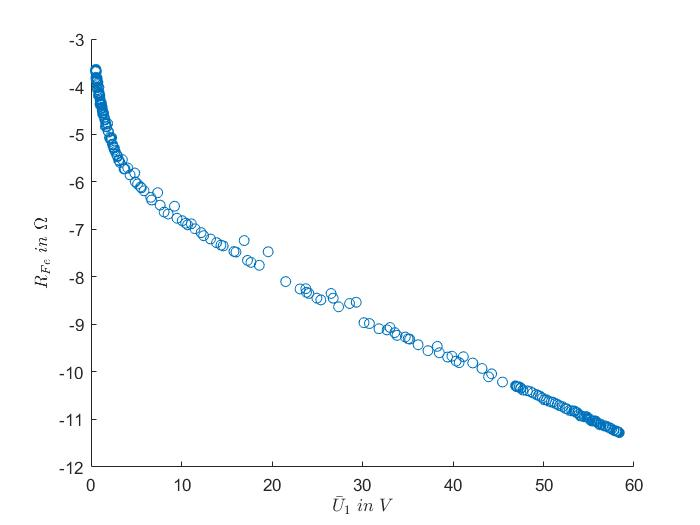
\includegraphics[width=\textwidth]{U1RFe1}
    \caption{Eisenwiderstand $R_{Fe}$ in Abhängigkeit von $\bar{U}_1$}
    \label{fig:}
  \end{subfigure}
  %
  \begin{subfigure}[b]{0.5\textwidth}
    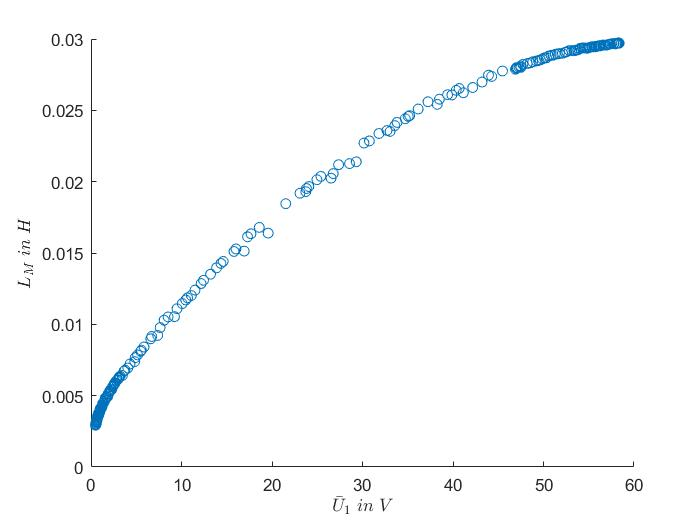
\includegraphics[width=\textwidth]{U1LM1}
    \caption{Hauptinduktivität $L_M$ in Abhängigkeit von $\bar{U}_1$}
    \label{fig:}
  \end{subfigure}
\end{adjustwidth}\centering
\begin{adjustwidth}{-1em}{7em}
  \begin{subfigure}[b]{0.5\textwidth}
    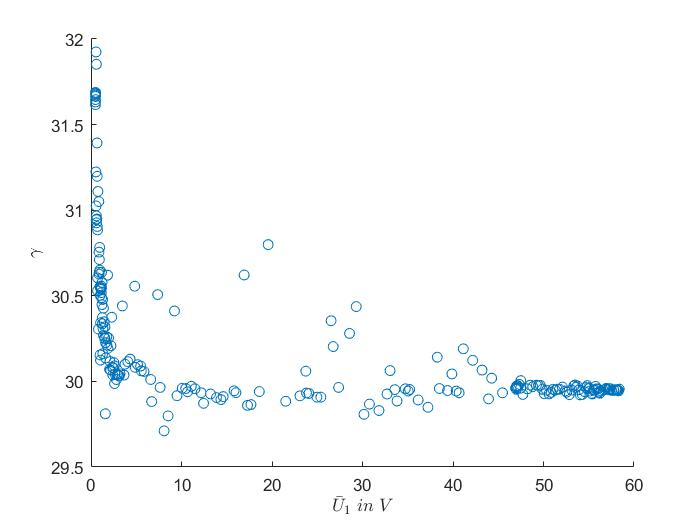
\includegraphics[width=\textwidth]{U11gam}
    \caption{Übertragungszahl $\gamma$ in Abhängigkeit von $\bar{U}_1$}
    \label{fig:}
  \end{subfigure} 
\end{adjustwidth}
\end{figure}
In der zweiten Messung hielten wir die Eingangsspannung konstant auf $\bar{U}_1=39.996\,V$. Durch Interpolation lassen sich für diesen Wert die Übertragungszahl $\gamma$, der Eisenwiderstand, die Hauptinduktivität, der Effektivwert der Stromstärke $I_{10}$ sowie die Phasenverschiebung $\varphi_{10}$ im Leerlauf bestimmen.
\begin{table}[H]\centering\begin{tabular}{ccccc}$\gamma$&$R_{Fe}$ in $\Omega$&$L_M$ in $H$&$\varphi_{10}$ in °&$I_{10}$ in A\\
29.994&9.721&0.026&130.298&0.0071\end{tabular}
\caption{Parameter der Stromkreises im Leerlauf für $\bar{U}_1=39.996\,V$}\end{table}
Die Ergebnisse der zweiten Messung sind in folgenden Diagrammen dargestellt.


Zur Berechnung des Innenwiderstands $R_i$, stelle ich zunächst eine Gleichung für die Ströme in der modifizierten Schaltung der Sekundärseite auf
\begin{align*}\gamma\,I_1=&\left(\frac{1}{R_i+R_L+i\,\omega\,L_\sigma}+\frac{1}{R_{Fe}}+\frac{1}{i\,\omega\,L_M}\right)\,\frac{U_1}{\gamma}\\
\Rightarrow\;\gamma^2\,\frac{I_1}{U_1}=&\gamma^2\,\frac{\bar{I}_1}{\bar{U}_1}\,e^{i\,\varphi_1}=\frac{1}{R_{Fe}}+\frac{R_i+R_L}{(R_i+R_L)^2+\omega^2\,L_\sigma^2}-i\left(\frac{\omega\,L_\sigma}{(R_i+R_L)^2+\omega^2\,L_\sigma^2}+\frac{1}{\omega\,L_M}\right)\\=:&|Y|\,e^{i\,\varphi_Y}\end{align*}
Daraus lassen sich folgende Gleichungen gewinnen.
\begin{align*}
|Y|\,\cos\varphi_Y=\gamma^2\frac{\bar{I}_1}{\bar{U}_1}\,\cos\varphi_1=\frac{1}{R_{Fe}}+\frac{R_i+R_L}{(R_i+R_L)^2+\omega^2\,L_\sigma^2}\\
|Y|\,\sin\varphi_Y=\gamma^2\frac{\bar{I}_1}{\bar{U}_1}\,\sin\varphi_1=-\left(\frac{\omega\,L_\sigma}{(R_i+R_L)^2+\omega^2\,L_\sigma^2}+\frac{1}{\omega\,L_M}\right)
\end{align*}
Hier besteht wieder das Problem, dass $\cos\varphi_1$ in dieser Messung negativ gemessen und damit korrigiert werden muss, und $\varphi_1$ ohnehin nur betragsmäßig bestimmt werden kann. Da in den Gleichungen prinzipiell nur positive Größen vorkommen muss $\varphi_1$ dann auch so gewählt werden, dass diesem Umstand Rechnung getragen wird. Für den Zweck einer einfacher nachzuvollziehenden Schreibweise benutze ich im folgenden Beträge, sodass sich die Gleichungen Umformen zu
\begin{align}
|Y|\,|\cos\varphi_Y|=\gamma^2\frac{\bar{I}_1}{\bar{U}_1}\,|\cos\varphi_1|=\frac{1}{R_{Fe}}+\frac{R_i+R_L}{(R_i+R_L)^2+\omega^2\,L_\sigma^2}\\
|Y|\,|\sin\varphi_Y|=\gamma^2\frac{\bar{I}_1}{\bar{U}_1}\,|\sin\varphi_1|=\frac{\omega\,L_\sigma}{(R_i+R_L)^2+\omega^2\,L_\sigma^2}+\frac{1}{\omega\,L_M}
\end{align}
Für den Strom $I_2$ gilt
\begin{align*}I_2=&\frac{1}{R_i+R_L+i\,\omega\,L_\sigma}\,\frac{U_1}{\gamma}\\
\Rightarrow\;\gamma^2\,\frac{\bar{I}_2^2}{\bar{U}_1^2}=&\frac{1}{(R_i+R_L)^2+\omega^2\,L_\sigma^2}
\end{align*}
Damit lassen sich Gleichungen(13) und (14) umschreiben zu
\begin{align*}
\gamma^2\frac{\bar{I}_1}{\bar{U}_1}\,|\cos\varphi_1|-\frac{1}{R_{Fe}}=(R_i+R_L)\,\gamma^2\,\frac{\bar{I}_2^2}{\bar{U}_1^2}
\end{align*}
Mit $R_L=U_2/I_2$ folgt daraus
\begin{align*}
R_i=\frac{\gamma^2\frac{\bar{I}_1}{\bar{U}_1}\,|\cos\varphi_1|-\frac{1}{R_{Fe}}}{\gamma^2\,\frac{\bar{I}_2^2}{\bar{U}_1^2}}-\frac{U_2}{I_2}
\end{align*}
$L_\sigma$ berechnet sich aus
\begin{gather*}
\gamma^2\frac{\bar{I}_1}{\bar{U}_1}\,|\sin\varphi_1|-\frac{1}{\omega\,L_M}=\omega\,L_\sigma\,\gamma^2\,\frac{\bar{I}_2^2}{\bar{U}_1^2}\\
\Rightarrow\;L_\sigma=\frac{\gamma^2\frac{\bar{I}_1}{\bar{U}_1}\,|\sin\varphi_1|-\frac{1}{\omega\,L_M}}{\omega\,\gamma^2\,\frac{\bar{I}_2^2}{\bar{U}_1^2}}\end{gather*}

\begin{figure}[H]\centering
\begin{adjustwidth}{-1em}{7em}
  \begin{subfigure}[b]{0.5\textwidth}
    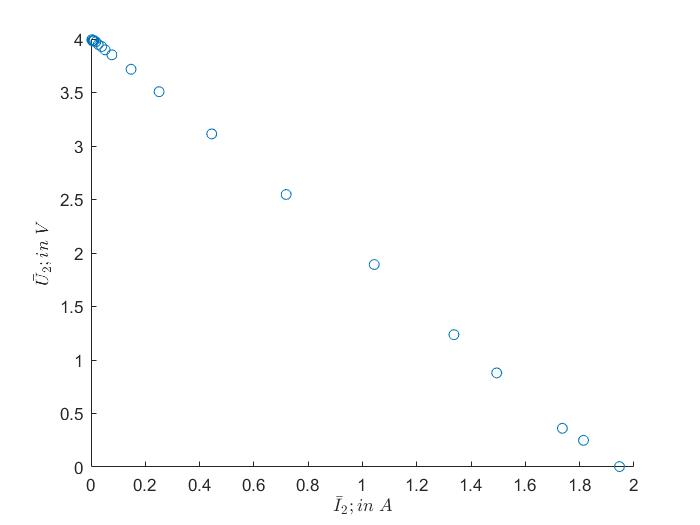
\includegraphics[width=\textwidth]{I2U22}
    \caption{Der Effektivwert der Spannung $\bar{U}_2$ in Abhängigkeit des Effektivwerts des Stroms $\bar{I}_2$}
    \label{fig:}
  \end{subfigure}
  %
  \begin{subfigure}[b]{0.5\textwidth}
    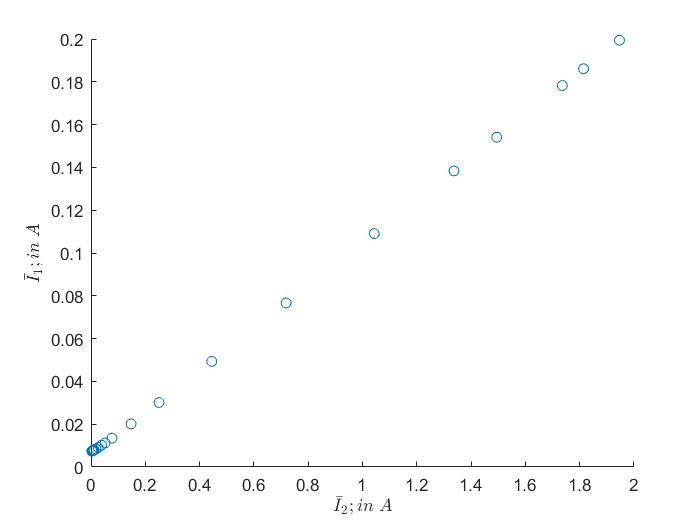
\includegraphics[width=\textwidth]{I2I1}
    \caption{Effektivwert des Stroms $\bar{I}_1$ in Abhängigkeit des  Effektivwerts der Stromstärke $\bar{I}_2$}
    \label{fig:}
  \end{subfigure}
\end{adjustwidth}\centering
\begin{adjustwidth}{-1em}{7em}
  \begin{subfigure}[b]{0.5\textwidth}
    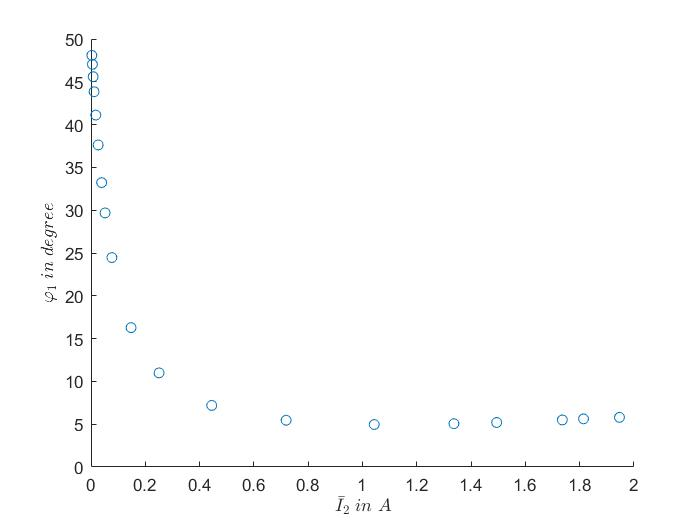
\includegraphics[width=\textwidth]{I2phi12}
    \caption{Phasenverschiebung zwischen Eingangsstrom und Eingangsspannung in Abhängigkeit von $\bar{I}_2$}
    \label{fig:}
  \end{subfigure} 
\end{adjustwidth}
\caption{Darstellung der Messwerte}
\end{figure}
Aus diesen Werten lassen sich nach obiger Ableitung der effektive Innenwiderstand und die effektive Streuinduktivität berechnen. Zur besseren Veranschaulichung habe ich die Werte logarithmisch gegeneinander aufgetragen.
\begin{figure}[H]\centering
\begin{adjustwidth}{-1em}{7em}
  \begin{subfigure}[b]{0.5\textwidth}
    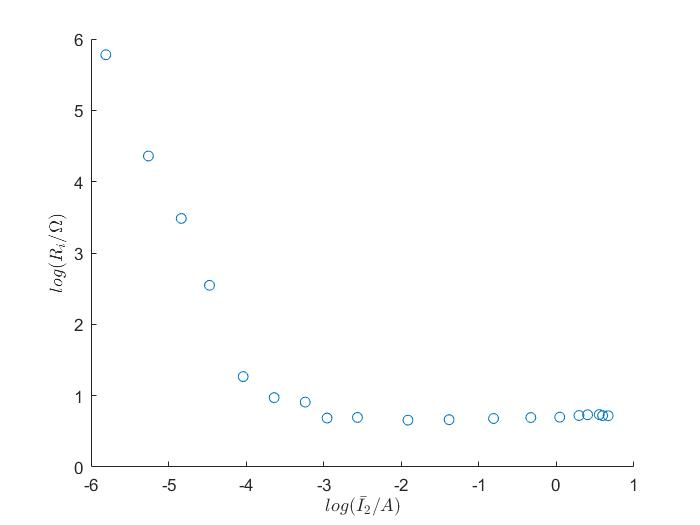
\includegraphics[width=\textwidth]{I2Rilog}
    \caption{Logarithmus des effektiven Innenwiderstands $R_i$ in Abhängigkeit des Logarithmus des Stroms $\bar{I}_2$}
    \label{fig:}
  \end{subfigure}
  %
  \begin{subfigure}[b]{0.5\textwidth}
    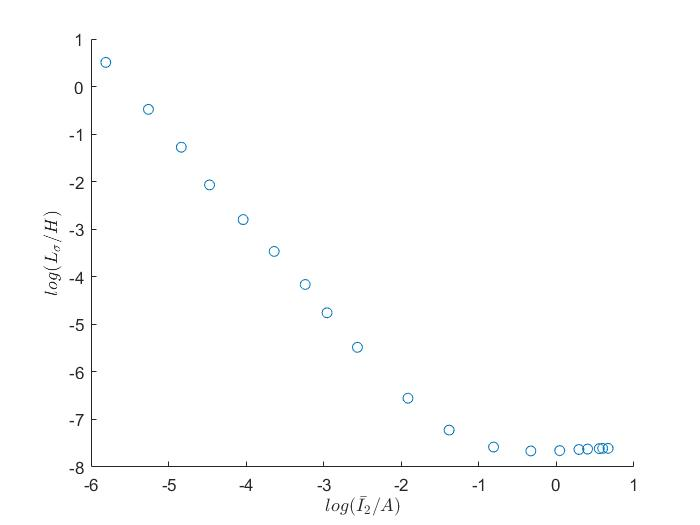
\includegraphics[width=\textwidth]{I2Lslog}
    \caption{Logarithmus der effektiven Streuinduktivität $L_\sigma$ in Abhängigkeit des Logarithmus des Stroms $\bar{I}_2$}
    \label{fig:}
  \end{subfigure}
\end{adjustwidth}\centering
\end{figure}
Wie in den Schaubildern zu erkennen ist, sind die Werte für einen Teil ziemlich konstant, bis sie für sehr kleine Ströme, d.h. sehr großen Lastwiderstand stark ansteigen. Dies erkläre ich mir dadurch, dass bei einem sehr großen Lastwiderstand die in Reihe geschalteten Innenwiderstand und Streuinduktivität einen verschwindend kleinen Effekt haben und dadurch schwer zu bestimmen sind. Deshalb mittele ich Innen Widerstand und Streuinduktivität über den Bereich in dem sie relativ konstant sind.
\begin{align*}R_i&=2.0147\pm0.1041\,(\text{stat.})\;\Omega\\
L_\sigma&=4.863\cdot10^{-4}\pm2.144\,(\text{stat.})\;H\end{align*}
Als Nächstes wird die Sekundäre Wirkleistung $\bar{P}_2=\bar{U}_2\,\bar{I}_2$ berechnet und dadurch der Wirkungsgrad berechnet.
\begin{figure}[H]\centering
\begin{adjustwidth}{-1em}{7em}
  \begin{subfigure}[b]{0.5\textwidth}
    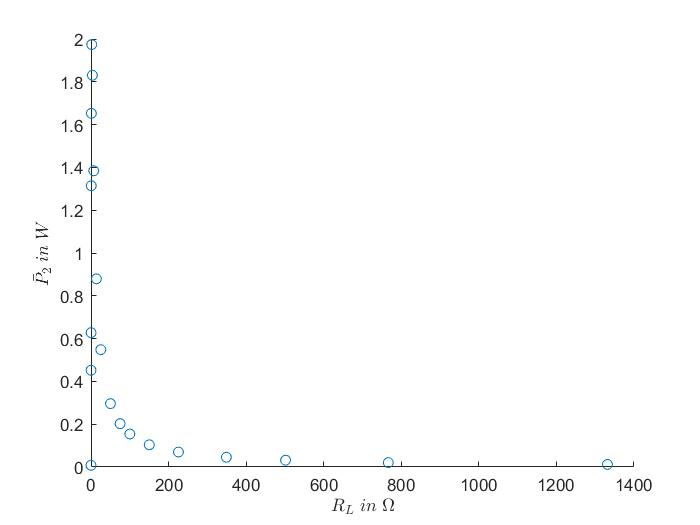
\includegraphics[width=\textwidth]{RLP2}
    \caption{sekundäre Wirkleistung in Abhängigkeit von $R_L$}
    \label{fig:}
  \end{subfigure}
  %
  \begin{subfigure}[b]{0.5\textwidth}
    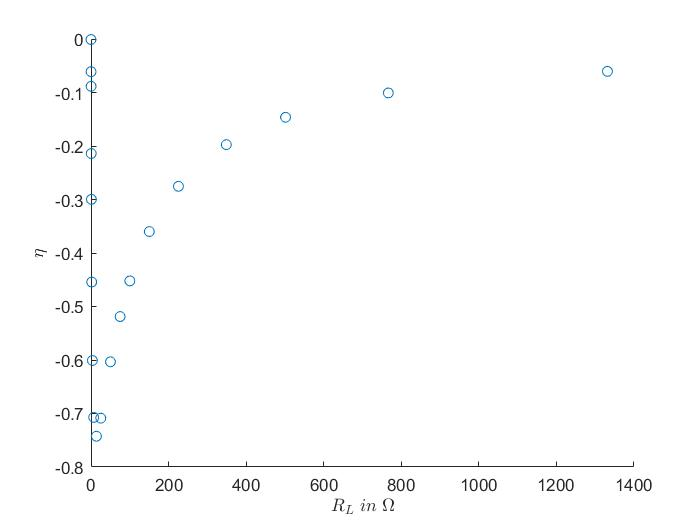
\includegraphics[width=\textwidth]{RLn}
    \caption{Wirkungsgrad $\eta=\bar{P}_2/\bar{P}_1$ in Abhängigkeit von $R_L$}
    \label{fig:}
  \end{subfigure}
\end{adjustwidth}\centering
\end{figure}
Der Verlauf der sekundären Wirkleistung und des Wirkungsgrads kann auch theoretisch aus den ermittelten Werten für die Schaltelemente des Transformators berechnet werden. Dafür müssen $\bar{P}_1$ und $\bar{P}_2$ bestimmt werden. Für $I_1$ gilt
\begin{align*}\gamma\,I_1&=\left(\frac{1}{R_{Fe}}+\frac{1}{R_i+R_L+i\,\omega\,L_\sigma}+\frac{1}{i\,\omega\,L_M}\right)\,\frac{U_1}{\gamma}\\
&=:Y\,\frac{U_1}{\gamma}\\
P_1&=U_1\,I_1=\frac{Y}{\gamma^2}\,U_1^2\\
\bar{P}_1&=\frac{\bar{U}_1^2}{\gamma^2}\,|Y|\,\cos\varphi_Y=\frac{\bar{U}_1^2}{\gamma^2}\,\mathfrak{Re}[Y]\\
&=\left(\frac{1}{R_{Fe}}+\frac{R_i+R_L}{(R_i+R_L)^2+\omega^2\,L_\sigma^2}\right)\,\frac{\bar{U}_1^2}{\gamma^2}\end{align*}
ähnlich bestimmt sich $\bar{P}_2$
\begin{align*}
I_2&=\frac{1}{R_i+R_L+i\,\omega\,L_\sigma}\,\frac{U_1}{\gamma}\\
&=:X\,\frac{U_1}{\gamma}\\
P_2&=U_2\,I_2=R_L\,I_2^2\\
\Rightarrow\;\bar{P}_2&=R_L\,|X|^2\,\frac{\bar{U}_1^2}{\gamma^2}\\
&=\frac{R_L}{(R_i+R_L)^2+\omega^2\,L_\sigma^2}\,\frac{\bar{U}_1^2}{\gamma^2}
\end{align*}












\end{document}